%\documentclass[11pt]{amsart}
\documentclass[review]{siamart}
\usepackage{geometry}                % See geometry.pdf to learn the layout options. There are lots.
\geometry{letterpaper}                   % ... or a4paper or a5paper or ... 
%\geometry{landscape}                % Activate for for rotated page geometry
%\usepackage[parfill]{parskip}    % Activate to begin paragraphs with an empty line rather than an indent
\usepackage{graphicx}
\usepackage{amssymb}
\usepackage{epstopdf}
\DeclareGraphicsRule{.tif}{png}{.png}{`convert #1 `dirname #1`/`basename #1 .tif`.png}

\title{Grid/cell services for gyrokinetic particle-in-cell simulations of highly magnetized plasmas}
\author{Mark F. Adams \and Tobin Issac \and Mathew Knepley}
%\date{}                                           % Activate to display a given date or no date
\nolinenumbers
\begin{document}
\maketitle

The simulation of highly magnetized fusion plasmas presents vast challenges in modeling, discretization, and efficient implementation on emerging architectures.
The Vlasov-Maxwell system with a collision operator on the right hand side is a 6D phase space set of equations and is, more or less, the basis of all numerical methods in plasma physics.
The gyrokinetic approximation is a common technique to reduce this to a 5D system.
The high dimensionality of this problem lends itself to particle-in-cell (PIC) methods although 5D continuum components are often hybridized with PIC in, for instance, the collision operator.
The strong magnetic guide fields, leading to highly anisotropic models with a large range of time and space scales, dominate the dynamics of fusion plasmas.
Engineering relevant predictive modeling of ITER plasmas is one of the great computational science challenges of today.

This document discusses a proposed contribution to this effort: developing fast, both algorithmically efficient and optimized for emerging architectures, solvers and related grid algorithms for PIC simulations of highly magnetized plasmas and deploying these methods to the public in the numerical library PETSc.
The PETSc project has a great deal of expertise and software for these services (e.g., discretizations, meshing and equation solvers).
This document presents a design of grid, or cell, methods, such as Poisson and implicit PIC solvers, gradients and charge deposition (particle-grid interaction), for PIC simulations.
We build on the Solver Integrated Tree-based Adaptive Refinement (SITAR) infrastructure in PETSc to provide services and abstractions useful for extreme-scale PIC applications.
In the following sections, the fundamental computational challenges are outlined, design requirements are enumerated, and an initial realization of an extreme-scale PIC data model and code is presented.

\section{Background}

Particle in cell (PIC) methods are effective approaches for discretizing high dimensional physics models in a variety of fields because of their lower cost on high dimensional problems relative to full grid or continuum methods.
PIC methods are naturally composed of three types of processing: 1) particle processing, the evolution of the 5D gyrokinetic Vlasov equation for magnetized plasmas, 2) grid processing, solvers, and 3) particle-grids interactions, charge deposition and gradients of potentials.
Most, say well over $99\%$, of the data in a PIC simulation of a fusion devise is in the particles.
Pure grid work, such as the Poisson solver, have abundant computational resources available and, for instance, can be run entirely on the CPU of accelerated architectures, or on a reduced set of cores on symmetric systems.
Note, the collision operator uses a 5D grid solve that is computationally demanding and fast solvers for emerging architectures are desired.
Pure particle processing, such as the ``push" of particles is relatively simple array processing.
Particle-grids interactions are challenging because the data structures and natural data decompositions are very different and are tightly coupled algorithmically.
The physics community has avoided some of this complexity by redundantly storing the entire field data (grid) on each MPI process or address space.
This data model is not tenable as we move to the exa-scale levels of parallelism required for engineering relevant ITER simulations.

The accurate and efficient simulations of these problems, to be of engineering relevance, for say the design and operation of ITER, is an extremely challenging problem.
The physics community has developed a large body of research and experience in using PIC methods for fusion plasmas and they are one of the largest users in DOE leadership class compute facilities.
The applied math, engineering, computational science, and physics communities have developed a great deal of expertise in discretization and solver methods for extreme-scale computing, but these advanced methods are not widely used in the fusion community.
The continued advancement of fusion simulations within DOE and the global community, especially as we move from reproducing known physics to engineering relevant predictive analysis, requires that both modern numerical methods and modern data decompositions and parallel computing techniques be employed.

These advanced methods require a large amount of engineering investment.
The goal of this work is to amortize these development costs, and the intellectual resources required to develop these algorithms, by developing an integrated solver, discretization, and meshing infrastructure in the widely deployed numerical library PETSc that provides grid services required by PIC codes, such as mesh generation, discretizations, fast equation solvers, and gradients and grid deposition at particle positions.
This work builds on SITAR in PETSc, which provides fast multigrid equations solvers that are tightly integrated with meshing and discretization of optimal efficiency on emerging architectures.
SITAR is bases on the {\it p4est} distributed tree library \cite{DBLP:journals/siamsc/IsaacBWG15,Rudi:2015:EIS:2807591.2807675,Stadler1033}.

\section{Design Requirements}

There are several general requirements for an extreme-scale fusion plasmas PIC application, which we would want supported by our work:
\begin{itemize}
\item Distributed memory data modes for particles and grids with good data locality relative to the solver mesh
\begin{enumerate}
\item Data locality for the deposit-solve-push process at the core of PIC algorithms
\item Independent flux tube grid for the collision operator
\end{enumerate}
\item Hierarchical grids for fast geometric multigrid solvers and adaptive mesh refinement
\item Abstract grid form physicists so that a variety of grids and discretizations can be used in the same code, often selected at run time
\item Incremental problems capacity, allowing for debugging and verification on simple grids (e.g., Cartesian grids) to full tokamak wall geometries
\item Fully convergent numerical methods that solve the given PDE with no free parameters other than those that explicitly appear in the equations (e.g., resistivities in resistive MHD)
\begin{itemize}
\item This requires particle shape factors or density smoothing to allow for arbitrary mesh resolution without increasing particle count to avoid particle noise and allows for code verification with rigorous convergence studies
\end{itemize}
\item A composable and extensible software design that allows for multiple algorithmic modules to be used, often as runtime parameters, within the same code
\begin{enumerate}
\item Grid discretizations (e.g., finite volume, finite element, discontinuous Galerkin)
\item Data decompositions and data models (e.g., redundant grid partitions, perhaps with redundant computation, to reduce communication)
\item Mesh methods (e.g., Cartesian, unstructured, flux surface following)
\item Architecture specific computational kernels for emerging architectures
\item Advanced programming models for emerging architectures \cite{KnepleyBrownMcInnesSmithRuppAdams2015}
\item Incremental contributions to the plasma physics community
\end{enumerate}
\end{itemize}

\section{Progress: An Extreme Scale PIC Code for Fusion Plasmas}

We have begun a PIC code to drive the developments proposed herein, to gather initial performance data on modern architectures to guide further developments, and to verify the implementations.
Our approach is to first exploit the fact that particle distributions, at least from a computational point of view, are relatively uniformly distributed over the domain and our grids are quasi-uniform; this allows for particle distributions that are simply attached to cells of the solver grid.
We use guide center particles only (i.e., only a parallel velocity, resulting in a 4D method).
These two simplifications allow us to reuse particle infrastructure that has been developed for other PETSc PIC users \cite{may2014ptatin}.
The collision operator, on the right hand side of Vlasov's equation, is a computational intensive non-linear solve in velocity space, which involves particles that interact with a certain collision frequency.
We simplify this process by partitioning particles into non-overlapping subdomains and compute collisions within these sets.
Flux tubes are the natural partitions for the collision operator; these are long, thin subdomains that follow the twisting magnetic field lines around the torus.
We currently repartition particles, which in the limit requires all particles be communicated, at the collision frequency.
This simplifies the implementation, because we can reuse the communications kernels used for the left hand side of Vlasov's equation, but future optimizations will most likely involve a more custom algorithm.
Note, one part of the philosophy of this development is to experiment, to base design decisions on data, and not relay only on one's intuition of a computer model for modern architectures.
Figure \ref{fig:cross} (left) shows an example of four flux tubes on a torus and Figure \ref{fig:cross} (right) shows an example of a coarse grid on a simple torus.
Note, the coarse grids of SITAR are unstructured and can accommodate a real tokamak geometry.
\begin{figure}[h!]
   \centering
   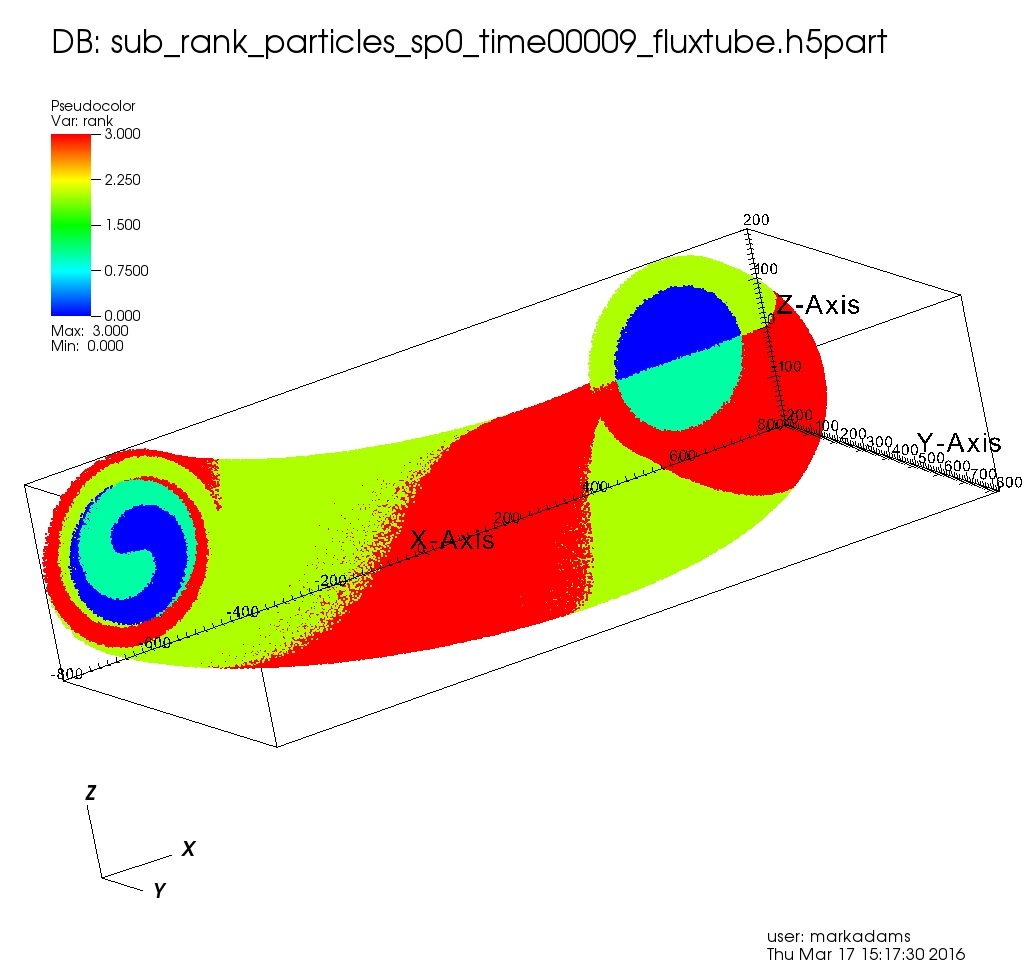
\includegraphics[width=75mm]{half_grid.jpeg} 
    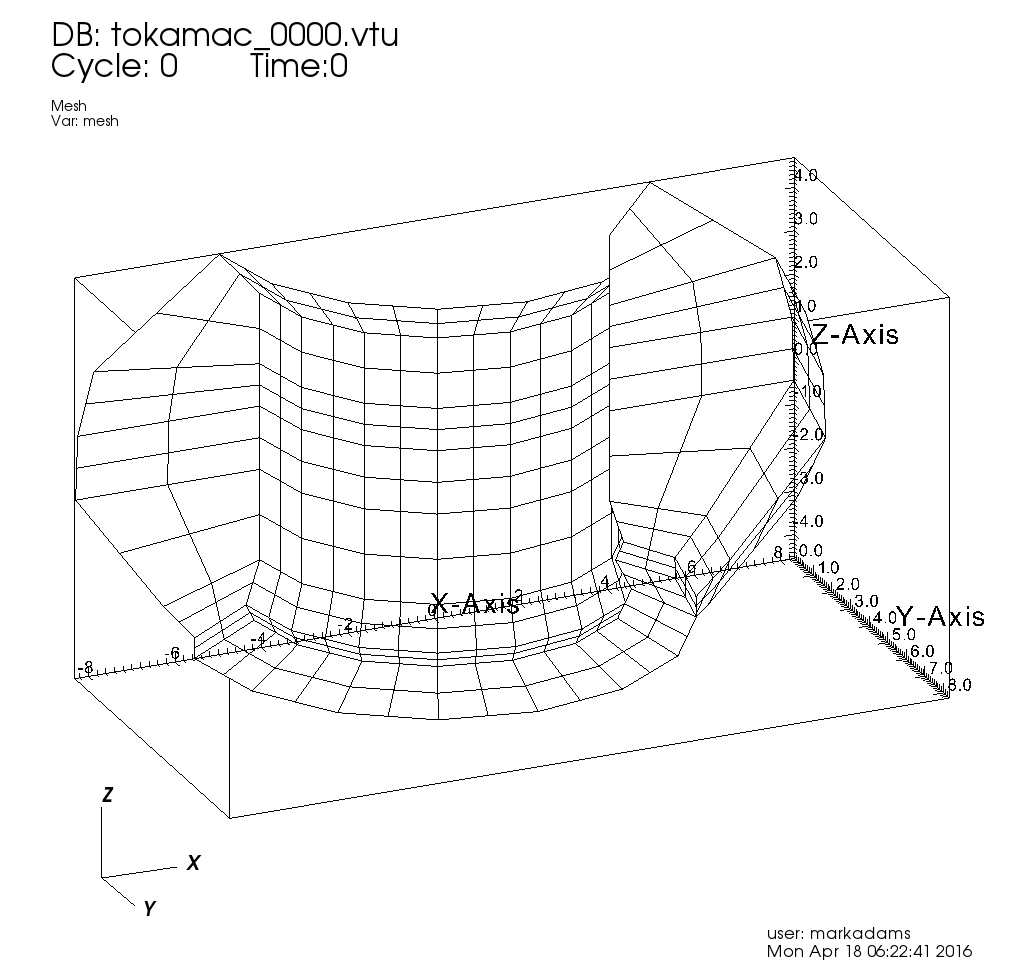
\includegraphics[width=75mm]{half_grid_mesh.jpeg} 
   \caption{Example 2x2x2 flux tube particle partition of torus (left); coarse grid solver mesh (right)}
   \label{fig:cross}
\end{figure}

The fuzzy edges of Figure \ref{fig:cross} (left) are due to the finite number of particles, each particle is drawn with the color of the partition to which it belongs.

\section{Future plans}

The realization of an engineering relevant full plasma simulation of ITER is a significant multi-year undertaking.
The development plans for this project are to be incrementally relevant and engaged with the physics community.
To this end early deliverables are important, to encourage physicists to participate and to stay grounded in the real engineering demands of this enterprise.
To this end we see two early areas that our project can contribute:
\begin{itemize}
\item Explore data decompositions and collect performance data to help further refine effective distributed data models for fusion PIC applications
\item Cross code verification of existing fusion PIC codes, without full physics, but with full ITER wall geometries
\end{itemize}
 
\bibliographystyle{siamplain}
\bibliography{./bib}


 
\end{document}  